\chapter{Softwaretechnik}

Zusammenfassung der Vorlesung "`Softwaretechnik 2"' aus dem Wintersemester 2016.\footnote{\url{https://sdqweb.ipd.kit.edu/wiki/Vorlesung_Softwaretechnik_II_WS16/17}}

\section{Einführung}

\section{Gesetzmäßigkeiten}
\begin{itemize}
	\item \textit{Brook's Law}: "`Adding manpower to a late software projcet makes it later."'
	\item \textit{Boehm's Law}: "`Errors are more frequent during requirements and design."'
	\item \textit{Dijkstra 1969}: "`Testing shows the presence, not the absende of bugs."'
	\item (One of) \textit{Lehman's Laws}: "`A system that is used will be changed."'
	\item \textit{Parnas' Law}: "`Only what is hidden can be chaned without risk"' (\(\rightarrow\) Kapselung notwendig)
\end{itemize}



\section{Software-Entwicklungsprozess}

\begin{itemize}
	\item "`Code and Fix"', als Vorgehensmodell unzureichend, da es zu schlecht strukturierten und dokumentierten Programmen führt
	\item Vorgehensmodell: Abstrakte Beschreibung eines Software-Entwicklungsprozesses. Beinhaltet Richtlinien bezüglich Aktivitäten, Rollen und Ergebnissen (Artefakte, Dokumente, etc.)
	\item \textbf{Wasserfallmodell}
	\begin{itemize}
		\item Phasen und Ergebnisse der Phasen
		\begin{enumerate}
			\item Planung: Lastenheft, Projektplan, Kalkulation
			\item Definition: Pflichtenheft, GUI-Beschreibung, eventuell Benutzerhandbuch
			\item Entwurf: Enwurfsdokumente, Modulführer
			\item Implementierung: Komponenten und Dokumentation, Testeinrichtung
			\item Testen
			\item Einsatz und Wartung: "`Fertiges"' System
		\end{enumerate}
		\item Probleme
		\begin{itemize}
			\item Große Softwareprojekte können i.d.R. nicht komplett (auf mehrere Jahre) geplant werden
			\item Abgrenzung der einzelnen Phasen in der Praxis oft unrealistisch
			\item Zu unflexibel bezüglich Änderungen oder Rückschritten
		\end{itemize}
	\end{itemize}
	\item \textbf{V-Modell} \\\\
		\begin{minipage}{\linewidth}
			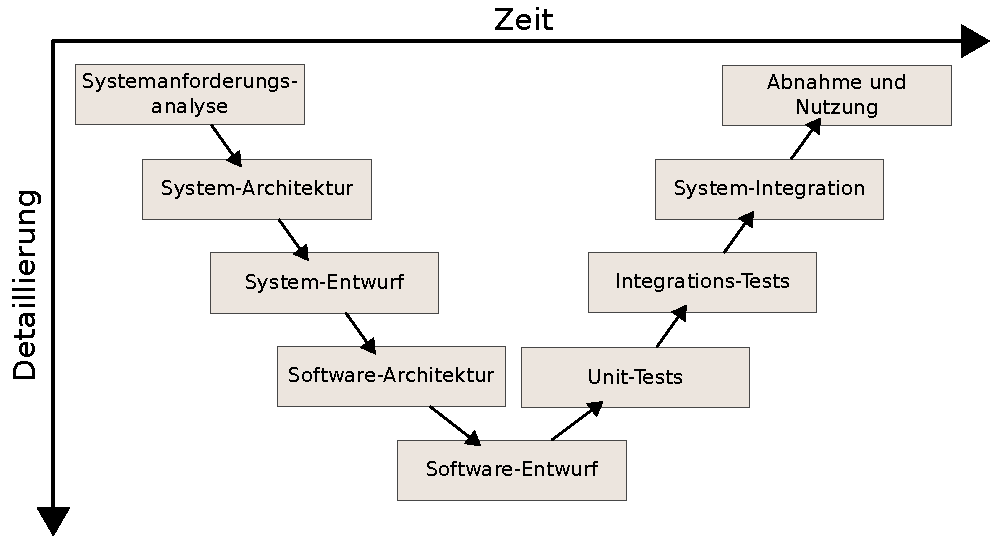
\includegraphics[scale=0.8]{swt2/v-modell.pdf}
		\end{minipage}
\end{itemize}



\section{Agile Entwicklung}

\subsection{Extreme Programming (XP)}
\begin{itemize}
	\item Sammlung aus Werten (Kommunikation, Einfachheit, Feedback, Mut) und Prinzipien (schnelle Lieferung/Feedback, Einfachheit) und Methoden
	\item \textbf{Der Prozess\footnote{\url{http://www.extremeprogramming.org/map/iteration.html}}}\\\\
		\begin{minipage}{\linewidth}
			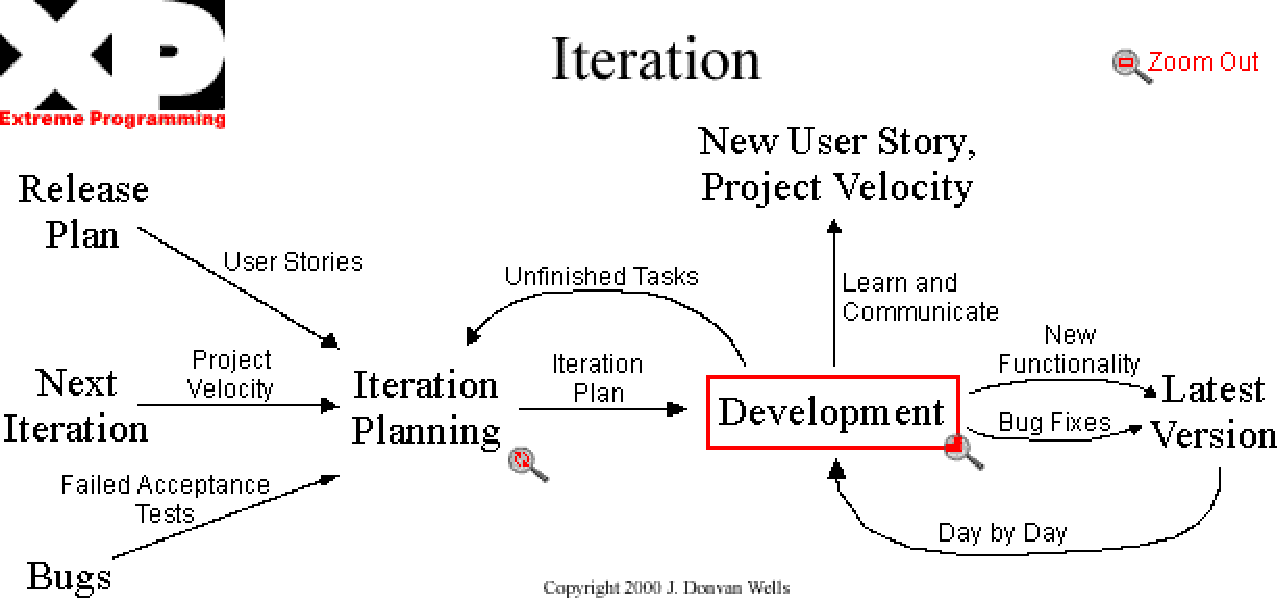
\includegraphics[scale=0.7]{swt2/xp_iteration.pdf}
		\end{minipage}
	\item \textbf{Kritik (allgemein auch an Agile)}
	\begin{itemize}
		\item Schlechte Skalierung bei großen Projekten
		\item Fehlende Dokumentation
		\item Kunden müssen aktiv mitarbeiten
		\item Wirksamkeit mancher Methoden nicht komplett überprüft (beispielsweise Pair-Programming)
	\end{itemize}
\end{itemize}


\subsection{Scrum}
\begin{itemize}
	\item \textbf{Zusammenfassung}
	\begin{itemize}
		\item \textit{Product Owner} erstellt/verwaltet eine priorisierte Liste mit Features, dem \textit{Product Backlog}
		\item Vor jedem \textit{Sprint} entscheidet das \textit{Team} welche Features in diesem \textit{Sprint} umgesetzt werden. Diese werden in den \textit{Sprint Backlog} übernommen
		\item Das \textit{Team} koordiniert die Entwicklung im täglichen \textit{Daily Scrum Meeting}. Der Fortschritt wird in einem Burn-Down-Chart festgehalten
		\item Der \textit{Srum Master} ist für die Kommunikation im \textit{Team} verantwortlich
		\item Während jedem \textit{Sprint} wird ein (möglichst) auslieferungsbereites \textit{Product Increment} erstellt
		\item Letzteres wird vom \textit{Team} im \textit{Sprint Review Meeting} vorgestellt. Anschließend werden im \textit{Retrospective Meeting} mögliche Verbesserungen besprochen
	\end{itemize}
	\item \textbf{Sprints}
	\begin{itemize}
		\item Idealerweise konstante Dauer von höchstens einem Monat
		\item Nach jedem Sprint startet direkt der nächste \(\rightarrow\) der Entwicklungsprozess besteht aus einer Folge von Sprints
		\item Während eines Sprint dürfen keine Änderungen gemacht werden, die das Ziel gefährden oder die Quailität verringern\\\\
		\begin{minipage}{\linewidth}
			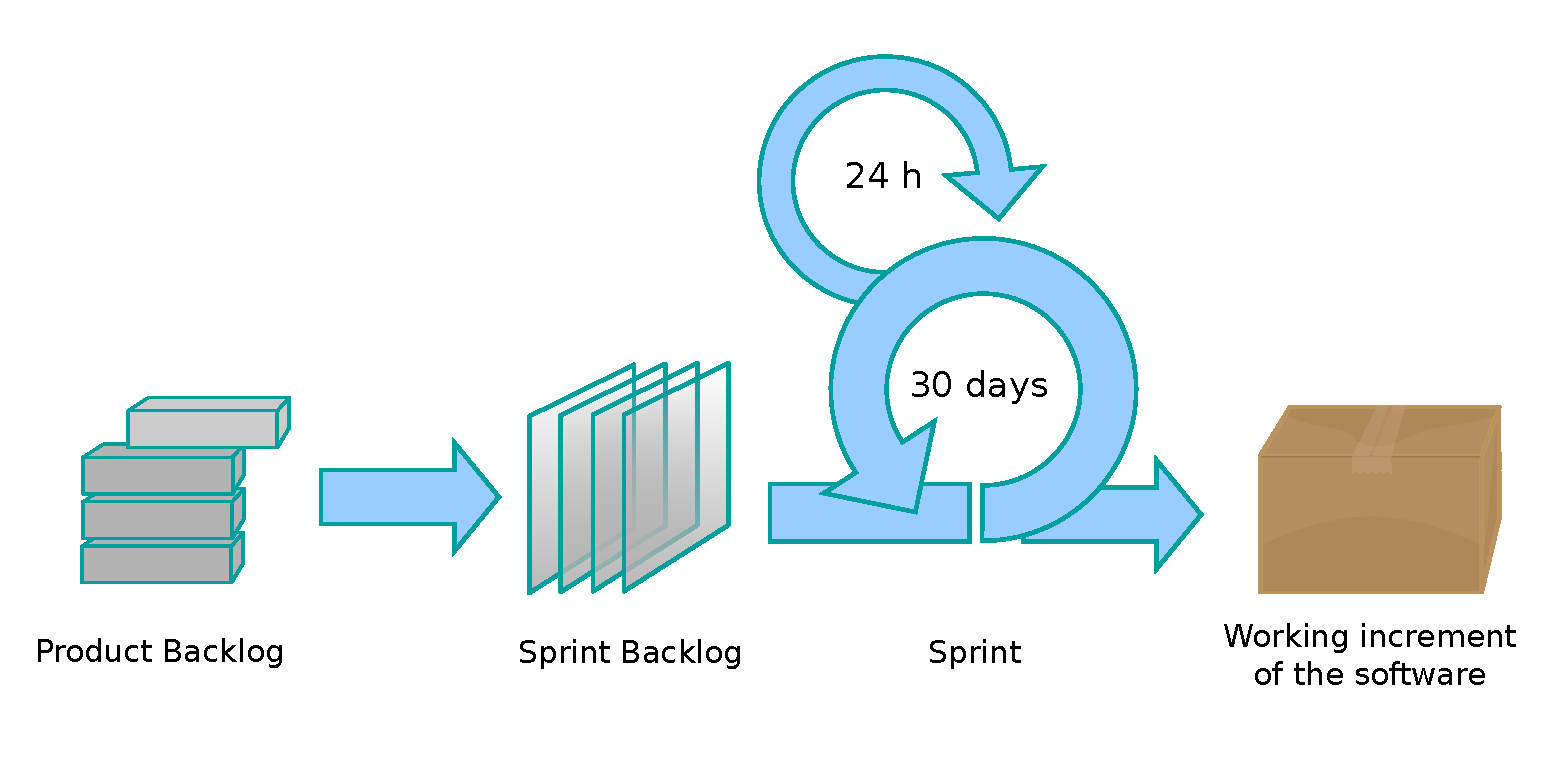
\includegraphics[scale=0.5]{swt2/scrum_process.pdf}
		\end{minipage}
	\end{itemize}
	\item \textbf{Aufgabenverteilung}
	\begin{itemize}
		\item Product Owner
		\begin{itemize}
			\item Repräsentiert den Kunden und ist für den wirtschaftlichen Erfolg des Produkts verantwortlich
			\item Erstellt/priorisiert/erklärt die Produkteigenschaften gegenüber dem Team
			\item Alleinverantwortlich für das Produkt
			\item Typische Fehler: Oft nicht verfügbar, zu wenig Durchsetzungskraft gegenüber unternehmensinternen Stakeholdern oder zu wenig technische Kenntnisse
		\end{itemize}
		\item Scrum Master
		\begin{itemize}
			\item Ist für die Umsetzung von Scrum verantwortlich
			\item Ist für die Kommunikation im Team verantwortlich
			\item Vermittelt gegenüber dem Product Owner
			\item Idealerweise ein Moderator, Coach und erfahrener Softwareentwickler
		\end{itemize}
		\item Team
		\begin{itemize}
			\item Selbstorganisierend, keine vordefinierten Rollen
			\item Idealerweise verschiedene Fachleute (GUI-Designer, Entwickler, Tester, etc.)
			\item Etwa sieben Vollzeitmitarbeiter
		\end{itemize}
		\item Kein klassischer Projektmanager vorhanden. Aufgaben werden von den drei Scrum-Rollen übernommen
	\end{itemize}
	\item \textbf{Product Backlog}
	\begin{itemize}
		\item Liste von Features, die alle Requirements beinhaltet. Nach Geschäftswert sortiert
		\item Jedes Element stellt eine User-Story da und beinhaltet eine Aufwandsangabe (\textit{Story Points})
	\end{itemize}
	\item \textbf{Sprint Backlog}
	\begin{itemize}
		\item User-Stories werden in kleinere Tasks aufgeteilt. Einzelner Task sollte nicht länger als 16 Stunden dauern
		\item Üblicherweise auf einer (non-)virtuellen Pinwand verwaltet \(\rightarrow\) bilden den Sprint Backlog
		\item Verschiedene Zustände pro Task. Beispielsweise: Todo \(\rightarrow\) In Arbeit \(\rightarrow\) Testen \(\rightarrow\) Fertig. Werden bei Zustandsänderung entsprechend verschoben/umgehängt
		\item Problem bei realen Pinwänden: Wissen geht eventuell nach Projektabschluss verloren
	\end{itemize}
	\item \textbf{Tipps für große Projekte}
	\begin{itemize}
		\item Teamgröße: Klein starten und organisch wachsen (siehe Brook's Law)
		\item Abhängigkeiten zwischen Teams verringern
		\item Daily "`Scrum of Scrums"' mit je einem (oder mehreren) Teammitgliedern
	\end{itemize}
	\item \textbf{Tipps für verteilte Teams}
	\begin{itemize}
		\item Nach Möglichkeit vermeiden
		\item Niemals Scrum Master und Team trennen
		\item Teams erst nach Eingewöhnung trennen
	\end{itemize}
\end{itemize}


\subsection{Zusammenfassung Agile Methoden}
\begin{itemize}
	\item Vorteile: Schnelles Feedback sowie reduzierte Risiken; hatte einen großen Einfluss auf Prozessverbesserung in der Industrie
	\item Nachteile: Verwenden der selben Codebasis in verschiedenen Projekten schwierig; Skalierung unklar; hoher Anspruch an die Entwickler; Dokumentation schwierig (Projekte teilweise nur im Code dokumentiert)
	\item Tendenziell Schwächen in Architektur und Design
\end{itemize}



\section{Anforderungsmanagement (Requirements Engineering)}

\subsection{Einführung}
\begin{itemize}
	\item 48 \% aller gescheiterten Softwareprojekte sind an mangelhafter Anforderungsdefinition gescheitert
	\item Beheben von falsch definierten Anforderungen in späteren Entwicklungsphasen kann extrem teuer sein
	\item Beschreibungskriterien: Ausreichend, komplett, widerspruchsfrei, verständlich, eindeutig, überprüfbar, risikoadjustiert
	\item Werden meist in Form von User-Stories (Agile) oder Anwendungsfälle (modellgetrieben) beschrieben
	\item \textbf{Typen von Anforderungen (concern-based Classification)}
	\begin{itemize}
		\item Funktionale Anforderungen (Functional Requirements): Verhalten der Software, beispielsweise bei der Eingabe von Daten; "`kann per Turing-Maschine beschrieben werden"'\footnote{Reussner, andere}
		\item Qualitätsanforderungen (Quality Requirements): Qualitätsmerkmale, beispielsweise Sicherheit, Bedienbarkeit, Performance
		\item Bedingungen (Constraints): Beispielsweise physikalische, rechtliche, kulturelle Umgebung oder Interface (Computerplattform)
	\end{itemize}
	\item Anforderungsingenieur vermittelt zwischen Entwicklern und Benutzern
	\item \textbf{Anforderungsmanagementprozess}
	\begin{enumerate}
		\item Gewinnung unter Einbeziehung sämtlicher Stakeholder
		\item Dokumentation: Anforderungsspezifikation aufstellen
		\item Übereinstimmung: Finden und Aufheben von Konflikten
		\item Überprüfen und Verwalten
	\end{enumerate}
\end{itemize}


\subsection{Techniken zum Finden von Anforderungen}
\begin{itemize}
	\item Fragetechniken: Interviews, Fragebögen, On-Site-Customers
	\item Kreativtechniken: Brainstorming, Perspektivwechsel
	\item Retrospektive Techniken: Systemüberreste, Wiederverwenden, Kokurrenzsysteme
	\item Beobachtungstechniken: Feldbeobachtungen
\end{itemize}

\subsection{Überprüfen ob Anforderungen umgesetzt sind}
\begin{itemize}
	\item Betriebsfähige: Reviews, Tests, formale Beweise
	\item Quantitative: Messen
	\item Qualitative: Keine direkte Prüfung möglich; eventuell (subjektiv) durch Jury
	\item Beschreibende: Reviews
\end{itemize}


\subsection{Grundlegende Beschreibungsempfehlungen}
\begin{itemize}
	\item Problem: Die meisten Anforderungen sind (zu Beginn) in natürlicher Sprache festgehalten
	\item Kurze Sätze, eine Anforderung pro Satz
	\item Festhalten wer für welche Aktionen/Handlungen verantwortlich ist
	\item Führen/Verwenden eines Begriffsglossars
	\item Verwenden einer Satzvorlage
\end{itemize}



\section{Modellgetriebene Entwicklung (Model Driven Development)}
\begin{itemize}
	\item Ziele: Plattformunabhängigkeit; höhere Entwicklungsgeschwindigkeit; bessere Softwarequalität; Wiederverwendbarkeit
	\item Erwartete Vorteile: Kostenreduzierung; kürzere Time-to-Market; variabel
\end{itemize}


\subsection{MDD-Paradigma}
\begin{itemize}
	\item \textit{Domain Expert} künftig für die Entwicklung von Anwendersoftware verantwortlich
	\item Modelle reduzieren die Komplexität, sind (automatisch) analysierbar, verbesseren die Kommunikationseffizienz
	\item \textit{Model-Driven}: Modelle sind primäre Artefakte, anstelle des Sourcecodes.
	\item \textit{Model-Based}: Modelle sind sekundäre Artefakte, die beispielsweise für Dokumentationen erstellt werden
\end{itemize}

\subsubsection{Beispiel: Model Driven Architecture (MDA)}
\begin{itemize}
	\item MDD Implementierung
	\item Bietet Standardisierung
	\item Verwendet existierende Standards
	\item \textbf{Modellformen}
	\begin{itemize}
		\item Computing Independent Models (CIM)
		\begin{itemize}
			\item Umgangssprachliche Beschreibung
			\item Klassendiagramm mit Klassenattributen aber ohne Klassenmethoden
		\end{itemize}
		\item Platform Independent Models (PIM)
		\begin{itemize}
			\item Plattformunabhängiges Modell für Geschäftsprozesse
			\item Hinzufügen von Methoden (und eventuell zusätzlichen, technischen Attributen) zum Klassendiagramm
		\end{itemize}
		\item Platform Specific Models (PSM)
		\begin{itemize}
			\item Plattformabhängiges Modell für Architektur/Services
			\item Ersetzen von generischen Typen durch plattformspezifische
		\end{itemize}
		\item Transformationen (Abstrakte Ebene \(\rightarrow\) Code-Ebene)\\\\
		\begin{tikzpicture}
			\node at (0, 0) [rectangle,draw] (cim)  {\(CIM\)};
			\node at (3, 0) [rectangle,draw] (pim)  {\(PIM\)};
			\node at (6, 0) [rectangle,draw] (psm)  {\(PSM\)};
			\node at (9, 0) [rectangle,draw] (code) {\(Code\)};

			\draw[->] (cim) edge node {} (pim);
			\draw[->] (pim) edge node {} (psm);
			\draw[->] (psm) edge node {} (code);
			\draw[<-] ($(pim.east)!0.5!(psm.west)$) -- ++(0,1cm) node[above] {Plattformmodell}; 
		\end{tikzpicture}
	\end{itemize}
\end{itemize}


\subsection{Schlüsselkonzepte und Definitionen}

\subsubsection{Metamodeling}
\begin{itemize}
	\item Vereinfachtes UML-Klassendiagramm
	\item Müssen immer vollständig sein, d.h. bereits alle Attribute/Typen und Assoziationen/Aggregationen enthalten, da sie automatisch weiterverarbeitet werden
\end{itemize}

\subsubsection{Model Transformation}
\begin{itemize}
	\item Transformation: \texttt{Meta-Model\_A} \(\longrightarrow\) \texttt{Meta-Model\_B} nach vorgegebenen Regeln
\end{itemize}


\subsection{Sprachen und Werkzeuge}
\begin{itemize}
	\item \textbf{Eclipse Modeling Framework (EMF)}
	\begin{itemize}
		\item De-facto MDD-Standard
		\item Wird von vielen großen Firmen und Projekten verwendet
	\end{itemize}
	\item \textbf{Essential Meta-Object Facility (EMOF)}
	\begin{itemize}
		\item Von der \textit{Object Management Group} (OMG) als Metadaten-Architektur definiert
	\end{itemize}
\end{itemize}

% TODO Rest ab Folie #48


\subsection{Forschung und Praxis}



\section{Designpatterns für Enterprise Application Architecture}
\begin{itemize}
	\item \textbf{Eigenschaften von Enterprise Applications (EA)}
	\begin{itemize}
		\item Langlebige Daten: Daten bleiben länger als Anwendungen und Hardware erhalten \(\rightarrow\) müssen in Anwendungen integrierbar sein
		\item Große Datenmengen mit meist mehreren Millionen Datensätzen \(\rightarrow\) effizienter Zugriff notwendig
		\item Konkurrierender Zugriff \(\rightarrow\) Inkonsistenzen müssen verhindert werden
	\end{itemize}
	\item Viele verschiedene Systeme: Shop, Leasing-Management-System, Ausgabenüberwachungssystem
	\item Web Shops: Viele parallele Anwender; einfache Logic
	\item \textbf{Ebenen}
	\begin{itemize}
		\item Präsentation: Benutzerinterface zur Informationsdarstellung und Eingabeverarbeitung
		\item Domain: Logik, Berechnungen
		\item Datenquelle: Kommunikation mit anderen Systemen, beispielsweise Datenbanken
	\end{itemize}
\end{itemize}


\subsection{Patternfamilien}
\begin{itemize}
	\item Jede Familie beschäftigt sich mit einem Problem von EAs
	\item Generell: Kein Pattern ist "`das beste"'. Wahl des Patterns aus einer Familie hängt von den konkreten Vorraussetzungen ab
\end{itemize}

\subsubsection{Domain-Logik Patterns}
\begin{itemize}
	\item Mögliche Herausforderungen: Hohe Komplexität, Austauschbarkeit, Verknüpfung mit Presentation und Datenquelle(n)
	\item \textbf{Pattern: Transaction Script}
	\begin{itemize}
		\item Jede Anfrage wird in einer separaten Prozedur abgearbeitet \(\rightarrow\) sämtliche Transaktionslogik in dieser Prozedur
		\item Beispiel: Laden von Objekt aus der Datenquelle, bearbeiten des Objekts, speichern des Objekts
		\item Vorteile: Einfache, verständliche Prozeduren; unkomplizierte Verbindungen mit Datenquellen; Transaktionsgrenzen einfach feststellbar
		\item Nachteile: Skalieren schlecht bei komplexer Logik; tendenziell doppelter Code
	\end{itemize}
	\item \textbf{Pattern: Domain Model}
	\begin{itemize}
		\item Objektmodell, das Verhalten und Daten beinhaltet
		\item Objekte arbeiten für Transaction zusammen
		\item Vorteil: Bessere Organisation der Domain-Logik
		\item Nachteile: Höhere Ansprüche an Entwickler; Mapping zur Datenquelle komplexer
	\end{itemize}
	\item \textbf{Pattern: Table Module}
	\begin{itemize}
		\item Einzelne Instanz, welche die komplette Logik für eine Tabelle implementiert
		\item Entweder eine Instanz pro Datensatz oder statisch per Singleton
		\item Vorteile: Einfaches Mappen Objekt \(\leftrightarrow\) Tabellenzeile; Logiktrennung für verschiedene Konzepte; nützlich, wenn von bereits verwendeten Technologien unterstützt
		\item Nachteil: Keine Instanzen pro Objekt \(\rightarrow\) eventuell unpraktisch/nachteilig bei komplexen Anwendungen
	\end{itemize}
	\item \textbf{Entscheidungskriterien}
		\item Wichtigstes Kriterium: Komplexität der Domain-Logik
		\begin{itemize}
			\item Bei wenig Komplexität: \texttt{Table Module < Transaction Skript < Domain Model} (gemessen am Implementierungsaufwand)
			\item Bei hoher Komplexität: \texttt{Domain Model < Table Module < Transaction Skript} (gemessen am Implementierungsaufwand)
		\end{itemize}
		\item Wie aufwendig ist das Mapping zur Datenquelle?
		\item Kennen die Entwickler das Domain-Model?
		\item Welche Werkzeuge/Entwicklungsumgebungen werden verwendet?
\end{itemize}

\subsubsection{Datenquelle-Architektur-Patterns}
\begin{itemize}
	\item Ziel: Trennung von Datenbankzugriff und Domain-Logic
	\item Herausforderung: Mapping Objekt \(\leftrightarrow\) Tabellenzeile
	\item \textbf{Pattern: Record Set}
	\begin{itemize}
		\item Lokale (in-memory) Kopie von Tabellenzeile(n)
		\item Einfach zu erzeugen und zu verändern
	\end{itemize}
	\item \textbf{Pattern: Table Data Gateway}
	\begin{itemize}
		\item Ein Objekt als Gateway (nicht als Facade), das den Zugriff auf alle Tabellenzeilen verwaltet
		\item Trennt Anfragen und Datenbankzugriff
		\item Implementiert \textbf{CRUD}-Methoden
		\item Geeignet für \texttt{Transaction Script}, eher ungeeignet für \texttt{Domain Model}
	\end{itemize}
	\item \textbf{Pattern: Active Record}
	\begin{itemize}
		\item Ein Objekt pro Tabellenzeile, das die Datenbankzugriff und Domain-Logic implementiert
		\item Objektorientiert: Vereint Daten und Funktionalität
		\item Mapping muss isomorph sein
		\item Gute Wahl bei wenig komplexer Domain-Logic, ansonsten ungeeignet \(\rightarrow\) \texttt{Data Mapper} verwenden
	\end{itemize}
	\item \textbf{Pattern: Row Data Gateway}
	\begin{itemize}
		\item Objekt, das als Gateway zu einer einzelnen Tabellenzeile fungiert
		\item Idee: Ähnlich wie \texttt{Active Record}, verhindert allerdings die Komplexität; kann SQL-Anfragen für verschiedene Datenbanktypen abstrahieren \(\rightarrow\) alle Zugriffsdetails sind hinter dem Interface versteckt
		\item Meist hat jede Tabelle eine Zusätzliche Finder-Klasse: \texttt{PersonFinder.find(id) \(\rightarrow\) PersonGateway}
		\item Gut geeignet für automatisch erzeugten Zugriffscode (der gesamte Datenbankzugriff wird generiert)
	\end{itemize}
	\item \textbf{Pattern: Identity Map}
	\begin{itemize}
		\item Jedes Objekt wird nur einmal aus der Datenbank geladen und dann lokal im Speicher vorgehalten (Cache)
	\end{itemize}
	\item \textbf{Pattern: Data Mapper}
	\begin{itemize}
		\item Mapping-Layer, der zwischen Datenbank und Objektspeicher vermittelt bzw. diese voneinander isoliert
		\item Mapping kann entweder explizit (für jedes Domain-Objekt existiert ein Mapper) oder Metadaten erfolgt werden, aus denen ggf. Code generiert wird
		\item Beispiel: \texttt{Hibernate}
		\item Verwendung
		\begin{itemize}
			\item Datenbankschema und Objekt-Modell entwickeln sich unabhängig (was meist der Fall ist)
			\item KomplexeBusiness-Logik, \texttt{Active Record} nicht ausreichend
			\item Automatisch erzeugt bei MDD
			\item Legacy Systeme mit bereits existierenden Datenbanken
		\end{itemize}
	\end{itemize}
\end{itemize}

\subsubsection{Sinnvolle Kombinationen aus Datenquelle-Pattern und Domain-Logic-Pattern}
\begin{itemize}
	\item \textbf{Transaction Script}
	\begin{itemize}
		\item \texttt{Row Data Gateway} oder \texttt{Table Data Gateway}
	\end{itemize}
	\item \textbf{Domain Model}
	\begin{itemize}
		\item Wenig komplexes Mapping: \texttt{Active Record}
		\item Komplexes Mapping: \texttt{Data Mapper}
	\end{itemize}
	\item \textbf{Table Module}
	\begin{itemize}
		\item \texttt{Table Data Gateway} (falls RecordSet-Framework)
	\end{itemize}
\end{itemize}

\subsubsection{Object-Relational Structural Patterns}
\begin{itemize}
	\item Mapping von OO-Strukturen zu relationalen Datenbanken (besonders bei \texttt{Domain Model} und \texttt{Data Mapper})
	\item \textbf{Pattern: Single Table Inheritance}
	\begin{itemize}
		\item Verherbungshierarchie mehrerer Klassen wird in einer einzigen Klasse repräsentiert, die Spalten für alle Attribute der verschiedenen Klassen und eine Type-Spalte hat
		\item Vorteile: Einfaches Datenbankschema; keine \texttt{Joins} notwendig; Verschieben von Attributen innerhalb der Hierarchie erfordert kein Anpassen der Tabelle
		\item Nachteile: Viele ungenutzte Attribute; Tabelle kann sehr groß werden; es gibt nur einen Namespace für alle Attribute (problematisch, falls mehrere Klassen gleiche Attributnamen für verschiedene Typen benutzen. Abhilfe: Naming Convention wie beispielsweise \texttt{[Classname]\_[Fieldname]})
	\end{itemize}
	\item \textbf{Pattern: Class Table Inheritance}
	\begin{itemize}
		\item Vererbungshierarchie mit je einer Tabelle pro Klasse
		\item Bei vererbten Klassen werden jeweils lediglich die neuen Attribute in der entsprechenden Tabelle gespeichert
		\item Vorteile: Einfach verständlich; Alle Spalten sind wichtig - keine Speicherverschwendung; einfaches Mapping zwischen Objekt und Datenbank
		\item Nachteile: Beim Laden eines Objekte müssen meist Daten aus mehreren Tabellen geladen werden (Leistungsverlust); aufwendigeres Refactoring; Supertypes können zum Flaschenhals werden
	\end{itemize}
	\item \textbf{Pattern: Concrete Table Inheritance}
	\begin{itemize}
		\item Jede Klasse der Vererbungshierarchie erhält eine Tabelle mit allen (auch den vererbten) Attributen
		\item Vorteile: Einfaches Zugriff, keine überflüssigen Spalten; keine \texttt{Joins} notwendig
		\item Nachteile: Verschieben von Attributen in der Hierarchie erfordert Schemaanpassung; Anpassungen bei Supertypes erfordern viele Änderungen; \texttt{find} über die Superklasse erfordert Suche in allen Subklassen (und damit Subtabellen)
	\end{itemize}
	\item \textbf{Verwendung}
	\begin{itemize}
		\item Alle Pattern in erster Linie zur Verwendung von \texttt{Domain Model} mit \texttt{Data Mapper}
		\item Abwägung zwischen Datendopplung und Geschwindigkeit
		\item Konkrete Wahl hängt von Zugriffsmustern ab
	\end{itemize}
\end{itemize}


\subsection{Praxis: Java Persistance API (JPA)}
\begin{itemize}
	\item Bestandteil von \texttt{Java EE}
	\item Definiert das komplette Mapping zwischen Objekt-Modell und Datenbank
	\item Kann wahlweise per \texttt{Java Annotations} oder \texttt{XML} definiert werden
	\item Vererbungspattern kann explizit festgelegt werden
\end{itemize}



\section{Software Design}

\subsection{Responsibility-Driven Design}
\begin{itemize}
	\item Zentrale Frage: Wie wird die Funktionalität auf die Objekte verteilt?
	\item Software-Objekte sollen tatsächlichen Objekten in der Realität entsprechen
	\item \textbf{Objekte erhalten \textit{Verantwortlichkeiten} (Responsibilities)}
	\begin{itemize}
		\item Doing responsibilities: Für welche Handlungen ist das Objektverantwortlich?
		\item Knowing responsibilities: Welche Informationen hält/teilt das Objekt
	\end{itemize}
	\item Verantwortlichkeiten werden mittels \texttt{Methoden} implementiert
	\item Pattern zum Verteilen von Verantwortlichkeiten: \textit{Informationsexperte}. Verarbeitung erfolgt in dem Objekt, das die Informationen hält
	\item Verarbeitungsbeispiel: Eingabeobjekt wird an die richtige "`Bearbeitungsstelle"' weitergegeben
\end{itemize}


\subsection{Design Diagramme}
\begin{itemize}
	\item Interaktionsdiagramme sind eine große Hilfe beim Entwurf
	\item Aus den fertigen Interaktionsdiagrammen können Software-Klassen abgeleitet werden: Nachricht im Interaktionsdiagramm \(\rightarrow\) Klassenmethode
	\item Typische Bestandteile eines Klassendiagramms: Klassen, Assoziationen, Attribute und deren Typen, Methoden, Interfaces, Abhängigkeiten
\end{itemize}


\subsection{General Responsibility Assignment Software Patterns (GRASP)}
\begin{itemize}
	\item Systematische Beschreibung, welche Objekte für was zuständig sein sollen
	\item \textbf{Creator}
	\begin{itemize}
		\item Legt fest, welches Objekt ein bestimmtes anderes erstellen soll
		\item \texttt{A} erstellt neues Objekt \texttt{B}, falls
		\begin{itemize}
			\item \texttt{A} eine Aggregation von \texttt{B} ist
			\item \texttt{A} \texttt{B}-Objekte beeinhaltet
			\item \texttt{A} \texttt{B}-Objekte mit starker Kopplung verwendet
			\item \texttt{A} die Initialisierungsdaten für \texttt{B} hat
		\end{itemize}
	\end{itemize}
	\textbf{Controllers}
	\begin{itemize}
		\item Der \texttt{Controller} oder \texttt{Facade} entscheidet, wie Ereignisse/Anfragen weiterverarbeitet werden
		\item Strategien
		\begin{itemize}
			\item Ein \textit{System Facade Controller}: Alle Ereignisse werden in dieser Klasse behandelt
			\item Ein Controller pro Anwendungsfall
		\end{itemize}
		\item Nicht gleichzusetzen mit einem \texttt{MVC}-Controller
	\end{itemize}
	\item Low Coupling: Niedriges Maß an Abhängigkeiten einer Klasse zu seiner Umgebung. Vereinfacht Änderungen und fördert Wiederverwendbarkeit und Verständlichkeit
	\item High Cohesion: Verringerung der Komplexität in dem unterschiedliche Funktionalität auf verschiedene Klassen aufgeteilt wird
	\item Polymorphism: Verwendung von polymorphen Klassen/Methoden statt \texttt{if} für verschiedene Eingabetypen. Erhöht allerdings die Gesamtzahl an Klassen/Methoden
	\item \texttt{Kompositionen > Vererbung}. \textit{Strategie-Pattern}: Verhalten wird zur Laufzeit konfiguriert
	\item Pure Fabrication: Normalerweise wird eine Pure Fabrication verwendet, um einen Algorithmus zu kapseln, der in keine Domain-Klasse passt. Sie kann zum Beispiel verwendet werden, um Technologiewissen von Domänenwissen zu trennen. Sie implementiert reines Verhalten und hat somit keinen Zustand. Sollte nicht zu häufig verwendet werden, sonst existieren am Schluss nur noch Klassen die einzelne Methoden kapseln.\footnote{\url{https://de.wikipedia.org/wiki/GRASP\#Pure_Fabrication}}
	\item Indirection: Indirection (Umweg) kann verwendet werden um geringe Kopplung zu erreichen. Sie wird erreicht, indem ein Vermittler zwischen Client und Server eingebaut wird. Sinnvoll wenn sich ein Serverobjekt ständig verändert. Als Nachteil ist die Leistungsfähigkeit vermindert. Beispielhaft für dieses Muster ist die Einführung der Controller-Komponente, die zwischen dem Datenmodell (Model) und dessen Präsentation (View) im Model-View-Controller-Architekturmuster vermittelt.\footnote{\url{https://de.wikipedia.org/wiki/GRASP\#Indirection}}
	\item Protected Variations: Interfaces sollen immer verschiedene konkrete Implementierung verstecken. Man nutzt also Polymorphismus und Delegation, um zwischen den Implementierungen zu wechseln. Dadurch kann das restliche System vor den Auswirkungen eines Wechsels der Implementierung geschützt werden.\footnote{\url{https://de.wikipedia.org/wiki/GRASP\#Protected_Variations}}
\end{itemize}



\section{Clean Code}
\begin{itemize}
	\item \textbf{Motivation}
	\begin{itemize}
		\item Schlechter Code senkt die Produktivität exponentiell
		\item Lesbarkeit extrem wichtig, da Code i.d.R. öfters gelesen als geschrieben wird
		\item Guter Code erhöht die Wartbarkeit ("`a system that is used will be changed"'\footnote{Lehman's first law} sowie "`an evolving system increases its complexity unless work is done to reduce it"'\footnote{Lehman's second law})
		\item Verwendung iterativer/inkrementeller Methoden (Agile) erreicht durch Refactorn, dass die Kurve flach bleibt
	\end{itemize}
\end{itemize}


\subsection{Die fünf SOLID-Prinzipien für gutes OO-Design}
\begin{enumerate}
	\item \textbf{Single Responsibility Principle (SRP)}
	\begin{itemize}
		\item Klassen sollen lediglich eine Verantwortung haben (Definition "`Anzahl Verantwortung"' über die Anzahl der Änderungsgründe)
		\item Bei komplexen Verantwortungen muss die Klasse ggf. aufgeteilt werden
		\item Verbessert die Lesbarkeit und verringert das Fehlerrisiko
	\end{itemize}
	\item \textbf{Open Closed Principle (OCP)}
	\begin{itemize}
		\item Softwareeinheiten sollen Erweiterungen möglich machen ohne ihr Verhalten zu verändern
		\item Beispielsweise durch Vererben und Überschreiben von Methoden
		\item Beispiel: Zeichnen verschiedener Grafikprimitiven
	\end{itemize}
	\item \textbf{Liskov Substitution Principle (LSP)}
	\begin{itemize}
		\item Ersetzbarkeitsprinzip fordert, dass eine Instanz einer abgeleiteten Klasse sich so verhalten muss, dass jemand, der meint, ein Objekt der Basisklasse vor sich zu haben, nicht durch unerwartetes Verhalten überrascht wird, wenn es sich dabei tatsächlich um ein Objekt eines Subtyps handelt\footnote{\url{https://de.wikipedia.org/wiki/Prinzipien_objektorientierten_Designs\#Liskovsches_Substitutionsprinzip}}
		\item Verletzung des Prinzips häufig nicht auf den ersten Blick erkennbar
	\end{itemize}
	\item \textbf{Interface Segregation Principle (ISP)}
	\begin{itemize}
		\item Dient dazu, große Interfaces aufzuteilen
		\item Die Aufteilung soll gemäß der Anforderungen der Clients an die Interfaces gemacht werden - und zwar derart, dass die neuen Interfaces genau auf die Anforderungen der einzelnen Clients passen. Die Clients müssen also nur mit Interfaces agieren, die das, und nur das können, was die Clients benötigen\footnote{\url{https://de.wikipedia.org/wiki/Prinzipien_objektorientierten_Designs\#Interface-Segregation-Prinzip}}
		\item Beispiel: Industrieroboter vs. Mensch. Ein Mensch benötigt mehr Zugriffe (essen, trinken,...)
	\end{itemize}
	\item \textbf{Dependency Inversion Principle (DIP)}
	\begin{itemize}
		\item Abhängigkeiten sollten immer von konkreteren Modulen niedriger Ebenen zu abstrakten Modulen höherer Ebenen gerichtet sein\footnote{\url{https://de.wikipedia.org/wiki/Prinzipien_objektorientierten_Designs#Dependency-Inversion-Prinzip}}
	\end{itemize}
\end{enumerate}


\subsection{Weitere Prinzipien}
\begin{itemize}
	\item \textit{Law of Demeter}: Objekte sollen nur mit Objekten in ihrer unmittelbaren Umgebung kommunizieren. Dadurch soll die Kopplung in einem Softwaresystem verringert und dadurch die Wartbarkeit erhöht werden\footnote{\url{https://de.wikipedia.org/wiki/Prinzipien_objektorientierten_Designs#Gesetz_von_Demeter}}
	\item \textit{Boy Scout Rule}: Code wird mit der Zeit schlechter \(\rightarrow\) regelmäßiges Refactern (beispielsweise vor dem Commiten)
	\item \textit{Principle of least Surprise}: Funktionen und Klassen sollten implementieren, was von ihnen erwartet wird (Intuitivität)
	\item \textbf{Code Conventions}
	\begin{itemize}
		\item Naming: Innerhalb eines Projekts/Teams standardisiert; aussagekräftig; Vermeidung unnötiger Pre-/Postfixes
		\item Commenting: Aussagekräftig; Verschieben von komplexen Kontrollstrukturen (die aufwendig kommentiert werden müssen) in Methoden
	\end{itemize}
	\item \textit{Don't repeat yourself} (DRY): Führt zu Fehlern und Inkonsistenzen. Vermindert Wartbarkeit, Verständlichkeit, Erweiterbarkeit
	\item \textit{Keep it simple (KISS)}: Erhöht die Verständlich. Beispiel: Verzicht auf unnötig komplexe Datenstrukturen
	\item \textit{You ain't gonna need it} (YAGNI): Features sind teuer/aufwendig (mehr Testing/Dokumentation). Implementiere lediglich was nötig ist
	\item \textit{Single Level of Abstraction} (SLA): Statements innerhalb einer Funktion/Funtionen innerhalb einer Klasse sollten auf dem selben Abstraktionslevel sein
	\item \textbf{Clean Architecture Patterns}
	\begin{itemize}
		\item 
	\end{itemize}
\end{itemize}


\subsection{Refactoring}
